%
%   TEMPLATE
%

\documentclass[11pt,b5paper,papersize,dvipdfmx]{jsbook}

\usepackage{vuccaken}
\usepackage{vuccaken2019}

% 以下本文 - - - - - - - - - - - - - - - - - - - - - - -
\begin{document}

% - - - - - - - - - - - - - - - - - - - - - - - - %
\kaishititle%
  {\LaTeX テンプレート(会誌原稿用)}% title
  {会計科学科4回生}% 所属
  {テンプレくん}% name
% - - - - - - - - - - - - - - - - - - - - - - - - %

% \setcounter{tocdepth}{2} % 目次にどこまで表示するか
% \tableofcontents % 目次出力
% \clearpage % 改ページ

%
\section*{はじめに}
実際に会誌にするときはjsbookクラスにしますが、面倒なので提出はこれでいいです。
テーマが複数ある場合は別ファイルで提出してください。\par
完成版の雰囲気は、去年までの会誌を見てください。

%
\section{セクション}
\subsection{サブセクション}
\subsubsection{サブサブセクション}
環境設定はこの前うpしたtex4tex.pdfにまとめてあります\footnote{Atomとかvscodeとかの高級エディタを使えば、シンタックハイライトだけでなく自動補完やショートカットなどもあって便利です。}。締め切りはSlackを見てください。\par
では、頑張ってください。

%
\section{てんぷれ!}

%
\subsection{数式}

%
\subsubsection{テイラー展開}
三角関数および指数関数のテーラー展開は次の通りである:
\begin{align}
    \cos x &= \sum_{n=0}^\infty \frac{(-1)^n}{(2n)!} x^{2n}, \label{eq:cos}\\
    \sin x &= \sum_{n=0}^\infty \frac{(-1)^n}{(2n+1)!} x^{2n+1}, \label{eq:sin}\\
    e^x &= \sum_{n=0}^\infty \frac{1}{n!} x^n. \label{eq:exp}
\end{align}

%
\subsubsection{オイラーの公式}
(\ref{eq:cos}),(\ref{eq:sin}),(\ref{eq:exp})式より
\begin{align*}
    e^{ix} = \sum_{n=0}^\infty \frac{1}{n!} (ix)^n
    &= \sum_{n=0}^\infty \frac{(-1)^n}{(2n)!} x^{2n} + i\sum_{n=0}^\infty \frac{(-1)^n}{(2n+1)!} x^{2n+1} \\
    &= \cos x + i\sin x
\end{align*}
よってオイラーの公式 $ e^{ix} = \cos x + i\sin x $ が示された。

%
\subsubsection{ギリシャ文字、数学記号}
ギリシャ文字とか記号は$\Gamma^\alpha_{\ \beta\gamma}, \Psi(x), \cos\theta, \sin^2\phi$や$\infty, \equiv, \approx, \to, \iff, \times, \cdots, \le$のように書きます。
変換でα, β, ∞, ×みたいにしないこと!

%
\subsection{グラフや画像の挿入}
\TeX はこれがめんどい。figure環境ごとコピペして使おう。

\begin{figure}[htbp]
  \centering
  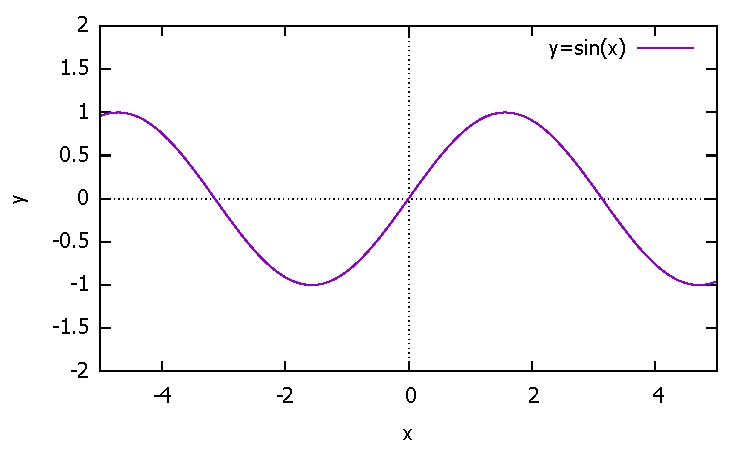
\includegraphics[width=10cm]{temp/fig-sin.pdf}
  \caption{$y=\sin x$のグラフ。gnuplotで作成した。}
  \label{fig:sin}
\end{figure}

図\ref{fig:sin}より、sinが{\bfseries うねうね}であることがわかる。

%
\subsection{箇条書き}
\begin{samepage}
  itemize: 番号なし
  \begin{itemize}
    \item 箇条書き
    \item できるやで
    \item[(a)] 平成最後で
    \item[ii)] おまんがな
  \end{itemize}
\end{samepage}

enumerate: 番号あり
\begin{enumerate}
  \item カブトムシ
  \begin{itemize}
    \item 美味しい
  \end{itemize}
  \item クワガタムシ
  \begin{enumerate}
      \item ギラファノコギリ
      \item ミヤマクワガタ
  \end{enumerate}
\end{enumerate}

%
\subsection{physicsパッケージ}
便利なphysicsパッケージのご紹介。煩雑な記号でもソースコードが簡潔です\footnote{詳しいマニュアルはターミナルで{\ttfamily texdoc physics}と打てば出てくるはずです。}。
\begin{align*}
  \dv{f}{x} (x), \dv{x} f(x), \pdv{f}{x} (x), \pdv{x} f(x),\\
  \dv[2]{f}{x} (x), \pdv[n]{x} f(x), \int \dd{x} g(x), \int \dd x g(x),\\
  \{ \frac12 \}, \qty{ \frac12 }, \qty( \frac12 ),\\
  \order{x^2}, \mqty(a & b \\ c & d), \mdet{a & b \\ c & d},\\
  \braket{\psi}, \braket{\phi}{\psi}, \ketbra{\phi}{\psi}, \hat n \ket{n}.
\end{align*}

%
\subsection{ascmacパッケージ}
枠で囲める。
\begin{itembox}[l]{定義(ゼータ関数)}
  $\Re(s) > 1$である任意の複素数$s$について、リーマンのゼータ関数$\zeta (s)$を以下のように定義する:
  \begin{align*}
    \zeta (s) := \sum_{n=1}^\infty \frac{1}{n^s}
    \equiv \frac{1}{1^s} + \frac{1}{2^s} + \frac{1}{3^s} + \frac{1}{4^s} + \cdots
  \end{align*}
\end{itembox}

%
\subsection{作図}
\LaTeX と連携できるものとしては、picture環境やTi{\itshape k}ZやgnuplotやInkscapeなど色々な方法がありますが、ここではキーワードを挙げるに留めておきます。
手描きを写真で撮ったり\footnote{明るさとコントラストをあげればそこそこキレイになる。}、パワポとかで作っても良いと思います\footnote{jpegは圧縮されて汚いので、pngか、ベクター形式のsvgとかpdfで作ると良い。}。

%
\subsection{ソースコード}
プログラムなどのソースコードを表示するにはlisting.styを使えばキレイに出力できますが、日本語に厳しい。そこで誰かが作ったplistings.styを代わりに使ってください。使い方はlisting.styと同じなので、そちらをキーワードにしてググってください。

%
\section*{参考文献}
\renewcommand{\labelenumi}{[\arabic{enumi}]} % [1],[2],...
\begin{enumerate}
  \item 著者, 本やページの名前, (URL), 出版社, 出版年.
  \item (複数ある場合は追加)
  \item @vuccaken, 物科研HP, \url{rp2017xy.starfree.jp}, 2019.
\end{enumerate}
\renewcommand{\labelenumi}{\arabic{enumi}.} % set to default


\end{document}
%
% ファイトだよ!
%